\documentclass{article}

% Language setting
% Replace `english' with e.g. `spanish' to change the document language
\usepackage[english]{babel}

% Set page size and margins
% Replace `letterpaper' with `a4paper' for UK/EU standard size
\usepackage[letterpaper,top=2cm,bottom=2cm,left=3cm,right=3cm,marginparwidth=1.75cm]{geometry}

% Useful packages
\usepackage{amsmath}
\usepackage{graphicx}
\usepackage[colorlinks=true, allcolors=blue]{hyperref}
\usepackage{float}
\usepackage{caption}
\usepackage{subfigure}

\title{lab02: Association Analysis -1}
\author{Group 18}


\begin{document}
\maketitle

This time we will try exploring monk1 dataset under the first vision of “monk problem”. Which is in short we have 5 attributes and 1 class label for each instance, and the label is classified by if (attribute 2 = attribute 1 or attribute 5 = 1) then class = 1, or else, class = 0.
\section{Clustering}

First, we will try clustering the dataset into 2 clusters via SimpleKmeans by L2 distance. Results are shown below:\\
\\
Within cluster sum of squared errors: 358.0 \\
\\
Classes to Clusters:\\
\\
  0  1  $<$-- assigned to cluster\\
 40 22 | 0\\
 37 25 | 1\\
\\
Cluster 0 $<$-- 0\\
Cluster 1 $<$-- 1\\
\\
Incorrectly clustered instances :	59.0	 47.5806 \% \\
\\

\begin{figure}[H]
\centering
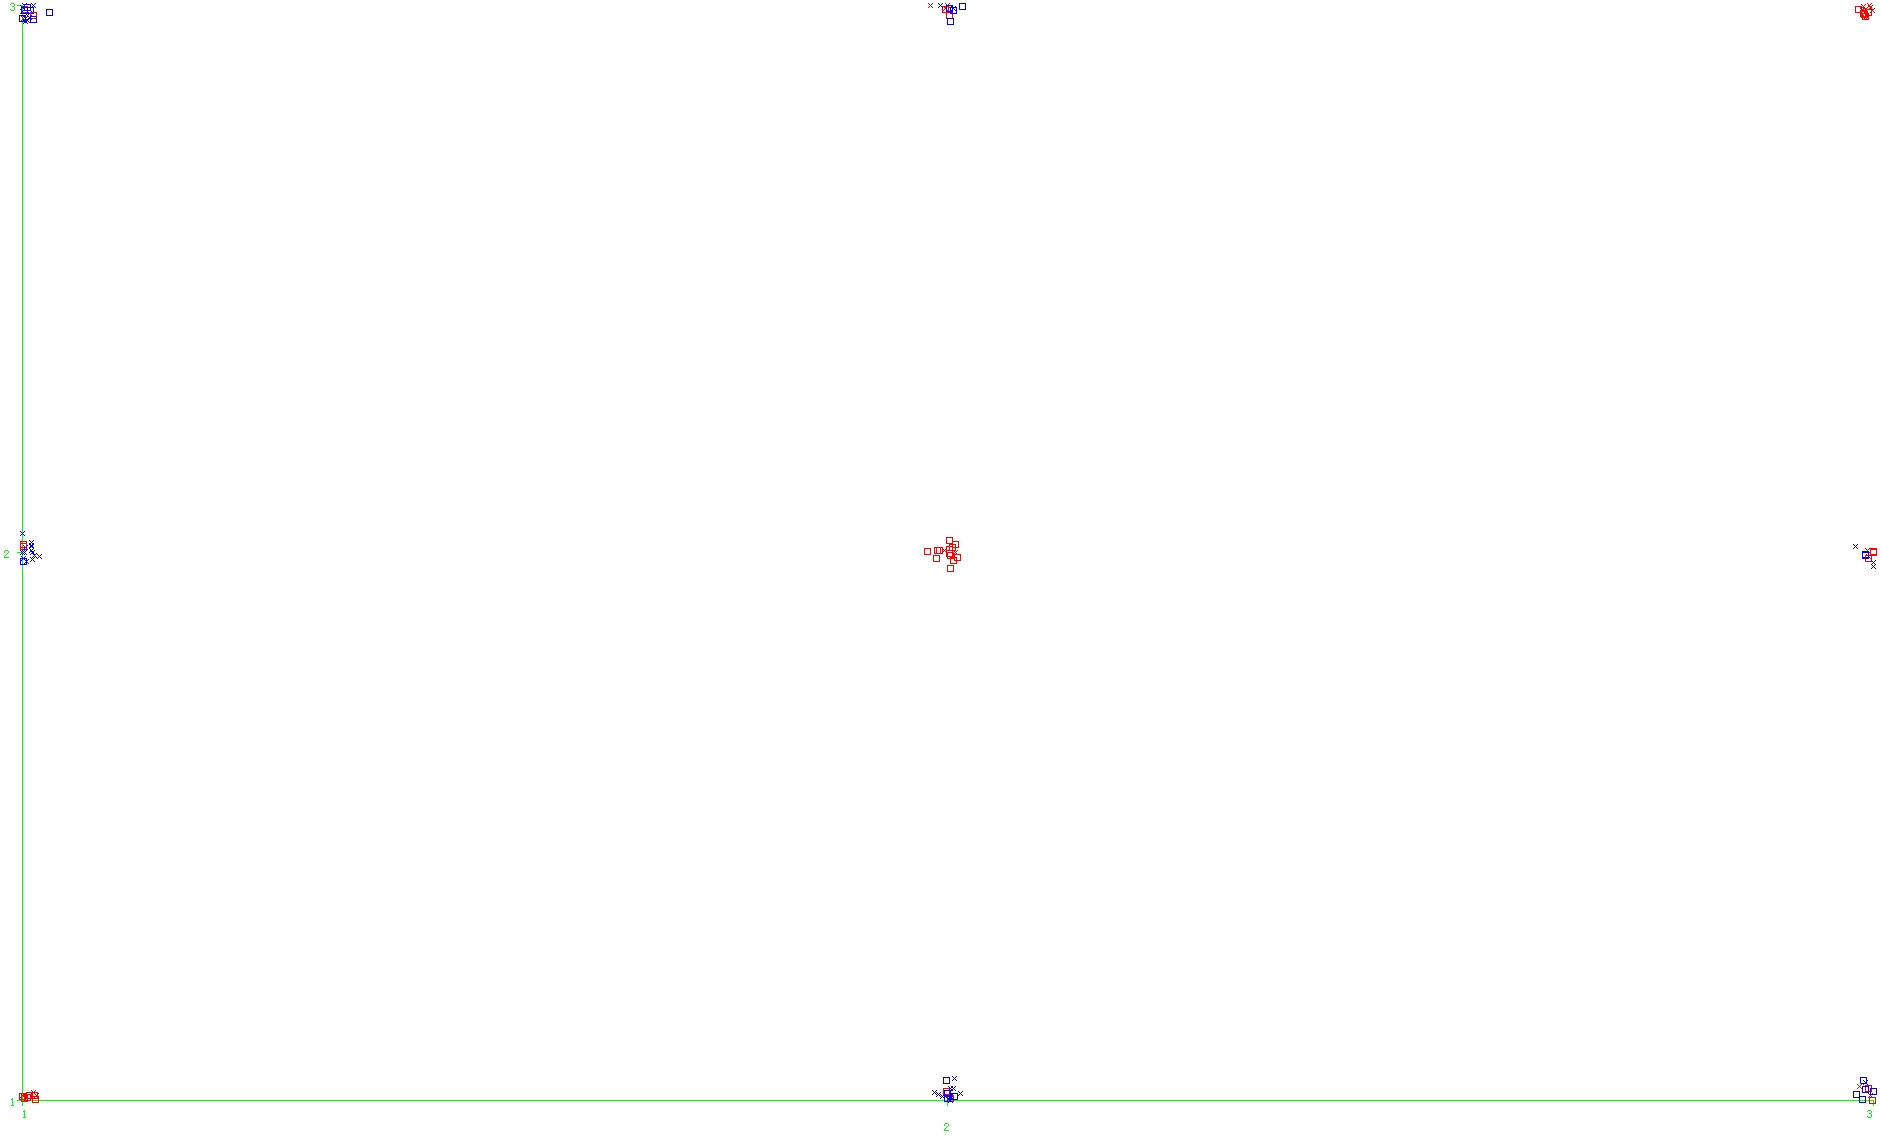
\includegraphics[width=0.8\textwidth]{kmeans2_x1VSx2_cClass.jpg}
\caption{\label{fig:kmeans2_x1VSx2_cClass}attribute 1 vs attribute 2 \\ color = class}
\end{figure}

Here we have an Incorrectly clustered rate of 47.5806 \% which has not much difference with 50\% and makes this clustering undesired, and the SSE 358.0 is also not so favorable. From the plot\ref{fig:kmeans2_x1VSx2_cClass} we can see that it’s a reasonable result. Clustering it into 2 clusters with such 2 feature dimensions by kmeans is impossible. It will need the algorithm to deal with non-convex clusters unless we raise the dimension.  Of course we have other dimensions to help. But even for the most prospective attribute 5, it have a great portion of class 1 evenly spread among value = 2 to 4(see plot\ref{fig:vis_x5_cClass}). Which we can expect it will make the result worse even it helps raises the dimension, let alone other attributes which contributes nothing by classification rules. To clarify this, we try same kmeans but changed the attrubutes used. From only using attribute 1 and 2, we got a 38.7097 \% Incorrectly clustered rate, then it becomes 45.9677 \% when adds attribute 5 in. And of course it’s 47.5806 \% when we add all attributes in.

\begin{figure}[H]
\centering
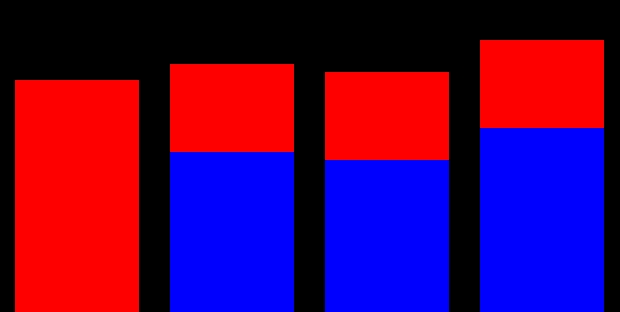
\includegraphics[width=0.8\textwidth]{vis_x5_cClass.jpg}
\caption{\label{fig:vis_x5_cClass}attribute 5 by value 1-4 \\ color = class}
\end{figure}

\section{Association analysis}

Then we proceed to association analysis using apriori algorithm with a minimum support of 0.05. Among the rules generated, we found 4 rules which can perfectly describe class 1:\\
\\
attribute\#5=1 29 ==$>$ class=1 29    conf:(1)\\
attribute\#1=3 attribute\#2=3 17 $==>$ class=1 17    conf:(1)\\
attribute\#1=2 attribute\#2=2 15 ==$>$ class=1 15    conf:(1)\\
attribute\#1=1 attribute\#2=1 9 $==>$ class=1 9    conf:(1)\\
\\
Despite there’re some overlapping instances simultaneously described by multiple(2) rules, we can perfectly describe class 1 by those 4 rules. And those which are not involved are all belongs to class 0.\\

\section{Conclusion}
As we discussed above, the data points belongs to different classes may tend to randomly  mixed with each other in the N-Dimension space when we have all the attributes(and even when we have only 3 necessary attributes). Thus clustering algorithm based on distance cannot work well on such problem. Instead, association analysis will work and oftenly makes the problem easier when dealing with high-dimension datasets than clustering.


\end{document}